\subsubsection{RFID}
\label{subsubsec:RFID}

Eine vorgesehene Funktion der Maschine ist, dass der User ohne Suchen sein Lieblingsgetränk zubereiten lassen kann. Dafür wird auf ein System zurückgegriffen, welches öfters für Zutrittskontrollen oder Ähnliches verwendet wird. Die Rede ist von RFID \footnote{Radio Frequency IDentification}.

Um schnell ein funktionierendes Teilsystem testen zu können, soll ein Breakout-Board verwendet werden. Eine Recherche hat ergeben, dass es für unseren Anwendungszweck nicht allzu viele Produkte gibt. Ein Eingrenzungskriterium war, dass es es für den Ausgewählten IC eine bestehende Library gibt, welche mit Arduino oder besser C kompatibel ist. Der Chip, welcher diese Anforderungen erfüllt, ist der \textbf{Mifare MFRC522}. Dieses Brakeout-Board kann ausserdem an der Verschalung der Maschine angeschraubt werden. Somit kann er sich an einer Stelle befinden, welche weiter weg von der Hauptsplatine ist.
Das Modul arbeitet auf 13.56MHz und gilt somit als kurzwelliges System (HF).

Der MFRC522 ist der Reader im RFID-System. Er kann Daten lesen und ggf. auch schreiben. Er erzeugt ein hochfrequentes, elektromagnetisches Wechselsignal mit einer Frequenz von 13.56MHz. Das Wechselfeld induziert beim Empfänger eine Spannung, welche als Energieversorgung dient. Durch Kurzschliessen der Tag-Antenne wird ein Teil der Energie des vom Reader ausgehenden Wechselfeldes verbraucht. Diese Energiedifferenz kann ein Reader detektieren.

Der Sender kann jedoch auch ein Datensignal über das Energiesignal modulieren. Die Informationen werden im Tag demoduliert und verwertet. Bei den Befehlen für den Tag geht es hauptsächlich um Lese- und Schreibmethoden. Bei einer Lesemethode des RFID wird ein Teil des Speichers abgefragt, bei Schreibmethoden wird der Speicher beschrieben. Die Reichweite für ein solches System, welches als Passivsystem deklariert ist, beträgt maximal 5cm.

Alternativ könnte ein Tag mit einer Batterie gespiesen werden. Somit erhöht sich die Reichweite des Readers, die Latenzzeiten werden kürzer und der Anwendungsbereich würde grösser. Solch ein System wird als Aktivsystem deklariert.

\paragraph{Schema}\mbox{}\\

Bild \ref{fig:Schema_RFID} zeigt den Schaltungsaufbau des RFID-Moduls. Darin ersichtlich sind folgende Teilbereiche:

\begin{itemize}
\item MFRC522 RFID IC
\item Antenne
\item Anpassnetzwerk für Antenne
\item Kommunikaitonsschnittstellen
\end{itemize}

\begin{figure}[!h]
\center
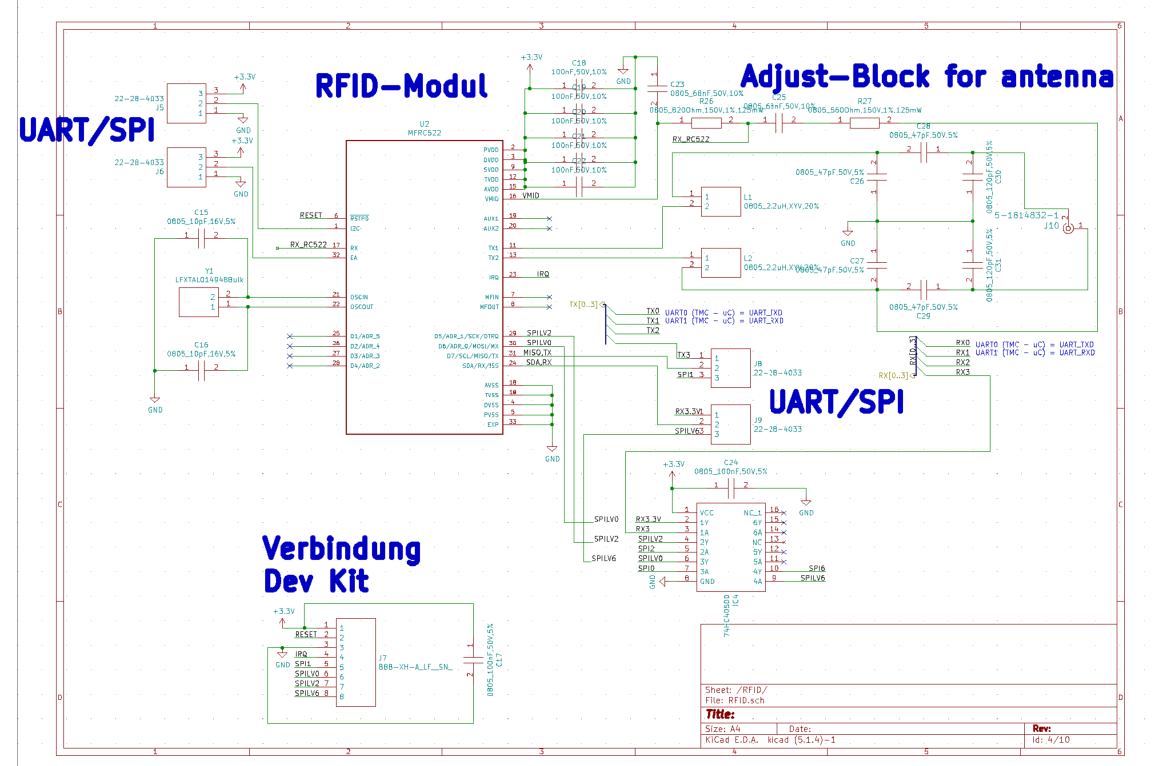
\includegraphics[width = 0.6 \textwidth]{graphics/Schema_RFID}
\caption{Schema des RFID Sender/Empfänger}
\label{fig:Schema_RFID}
\end{figure}

\paragraph{Funktionsbeschrieb der Schaltung}\mbox{}\\

Der IC steuert den Ablauf, damit die Datenübertragung stattfinden kann. Er verbindet die Antenne mit dem Cocktailmixer und liest bzw. schreibt die Informationen auf das bzw. aus dem Trägersignal. Die Herausforderung besteht im Design des Anpassnetzwerkes an das IC und die Antenne. Wie die Bauteile dimensionert werden, kann in einer Anleitung nachgelsen werden. Sie dazu Anleitung: \cite{nxp_bv_2010_antenna_2010}.

Die Anschlüsse sind so gestaltet, dass falls eine einens gelayoutete Antenne verwendet wird, die Kommunikation zwischen UART und SPI gewählt werden kann. Aus Zeit- und Backupgründen wurde für die Cocktailmaschine ein Breakout-Board verwendet, welches nur einen SPI-Anschluss hat. In erster Linie damit keine Zeit gebraucht wird, sich mit einem Antennendesign auseinandersetzen zu müssen. Aber auch, weil der IC in ein TQFP28-Gehäuse gepackt ist, und deshalb Schwierigkeiten auftreten könnten beim Löten.